\documentclass[11pt, oneside]{article}   	% use "amsart" instead of "article" for AMSLaTeX format
\usepackage{geometry}                		% See geometry.pdf to learn the layout options. There are lots.
\geometry{letterpaper}                   		% ... or a4paper or a5paper or ... 
%\geometry{landscape}                		% Activate for for rotated page geometry
%\usepackage[parfill]{parskip}    		% Activate to begin paragraphs with an empty line rather than an indent
\usepackage{graphicx}
\usepackage{amsmath}				% Use pdf, png, jpg, or eps§ with pdflatex; use eps in DVI mode
								% TeX will automatically convert eps --> pdf in pdflatex		
\usepackage{amssymb}

\title{Homework 7 - CS6210}
\author{Ally Warner}
%\date{}							% Activate to display a given date or no date

\begin{document}
\maketitle
\section{Grid}

Write a program to generate a 'finite difference grid' for the problem. This program should accept a value of h as input. To generate a grid means to break up the solution domain into uniform subregions and specifying the node points. It is acceptable to require that 1/h be an integer in order to avoid problems that arise when the boundary is not on a grid line. \\

To create my 'finite difference grid', I first calculated the size of the grid based on the input of $h$, which is the distance between nodes on our grid. I went through and plotted nodes from the bottom to the top of the grid, going left to right in each row. I saved the x and y positions of the nodes to be able to convert the grid into a matrix problem. I plotted my grid at five different values of $h$ shown in the following figures. The code to create the grid follows. \\

\centerline{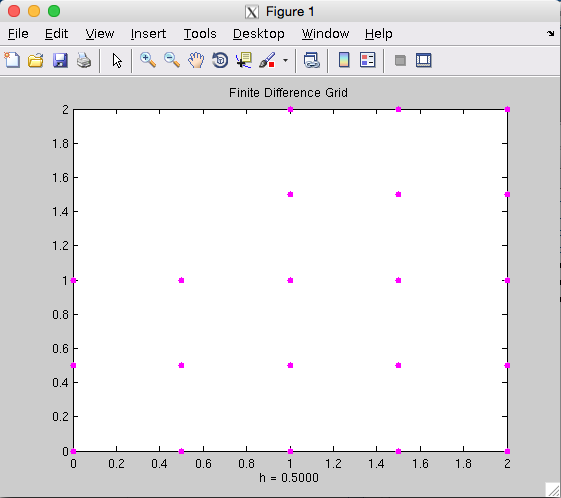
\includegraphics[scale = 0.55]{Grid_h1.png}}

\centerline{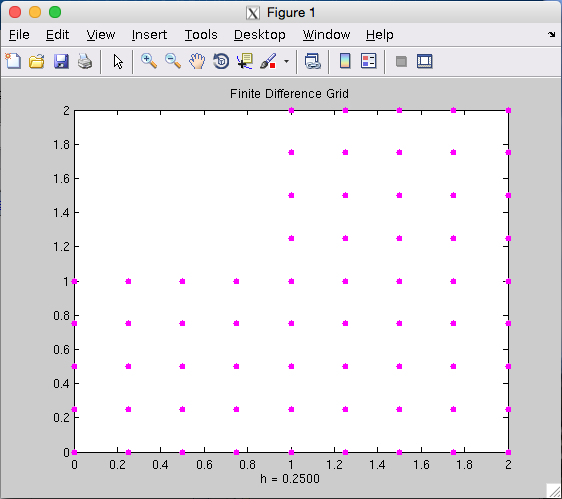
\includegraphics[scale = 0.55]{Grid_h2.png}}

\centerline{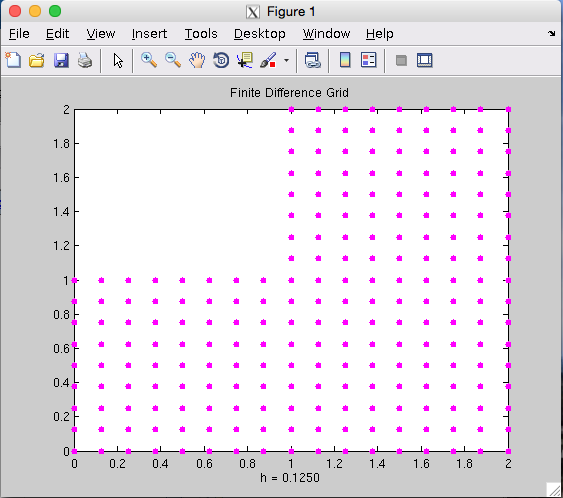
\includegraphics[scale = 0.55]{Grid_h3.png}}

\centerline{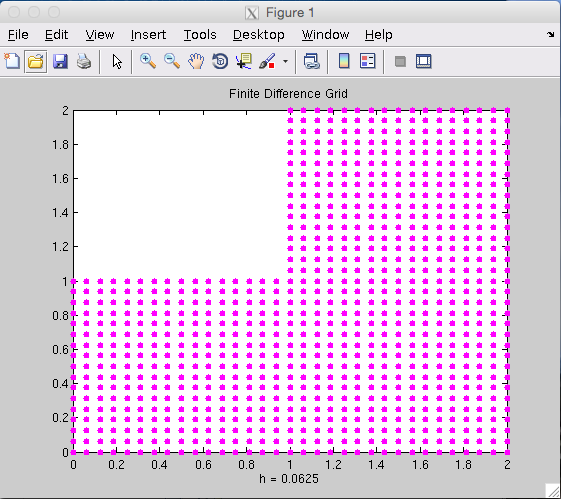
\includegraphics[scale = 0.55]{Grid_h4.png}}

\centerline{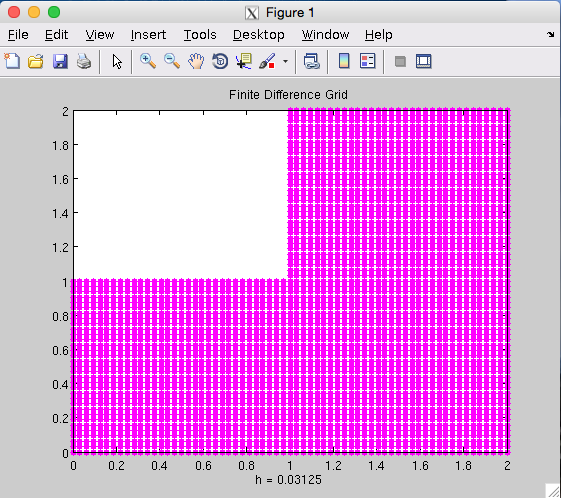
\includegraphics[scale = 0.55]{Grid_h5.png}}

\centerline{\includegraphics[scale = 0.7]{MakeGridCode.png}}

\section{Solving a Linear System}

Write a program to convert this grid into a matrix problem (a linear system Ax = b) using a 5 point centered difference finite difference approximation. \\

To convert my position information obtained from making the finite difference grid, I dealt with the bottom part of the region separately from the top part of the region to make the calculations easier to work with. Then for each case of node, weights were assigned to the current node and the four nodes surrounding. These weights were put into a matrix, $A$, where each row corresponds to a node. The solution matrix, $b$, was also created in this program based on the boundary conditions of our system. After $A$ and $b$ were constructed, I used the backslash operator in MATLAB to quickly solve this linear system and visualize my results. The results were visualized for five different values of $h$ shown in the following figures. The code to create the stencil follows. \\

\centerline{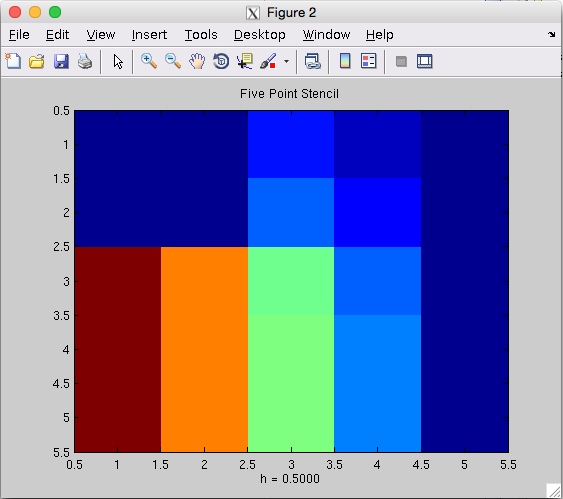
\includegraphics[scale = 0.55]{FivePoint_h1.png}}

\centerline{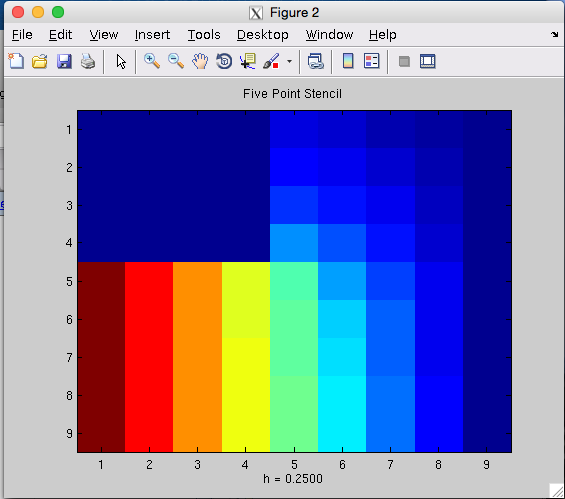
\includegraphics[scale = 0.55]{FivePoint_h2.png}}

\centerline{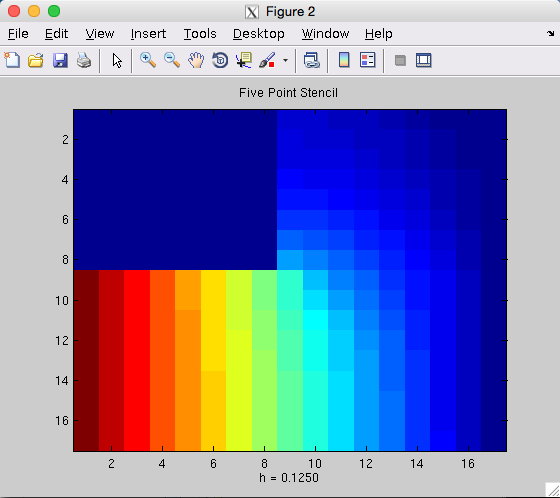
\includegraphics[scale = 0.55]{FivePoint_h3.png}}

\centerline{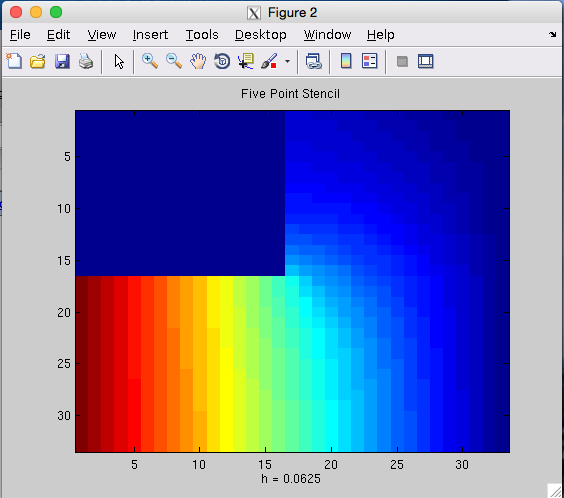
\includegraphics[scale = 0.55]{FivePoint_h4.png}}

\centerline{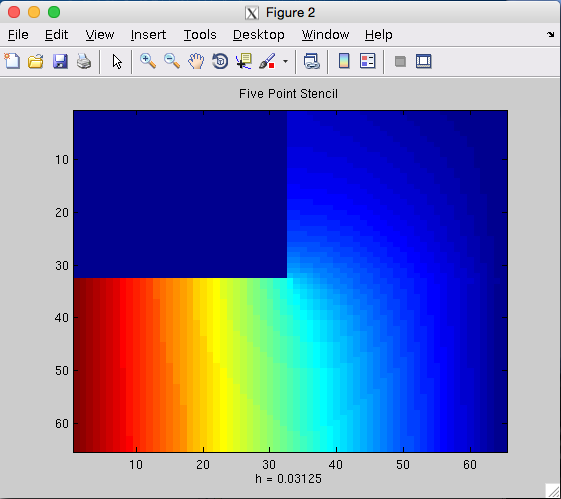
\includegraphics[scale = 0.55]{FivePoint_h5.png}}

\centerline{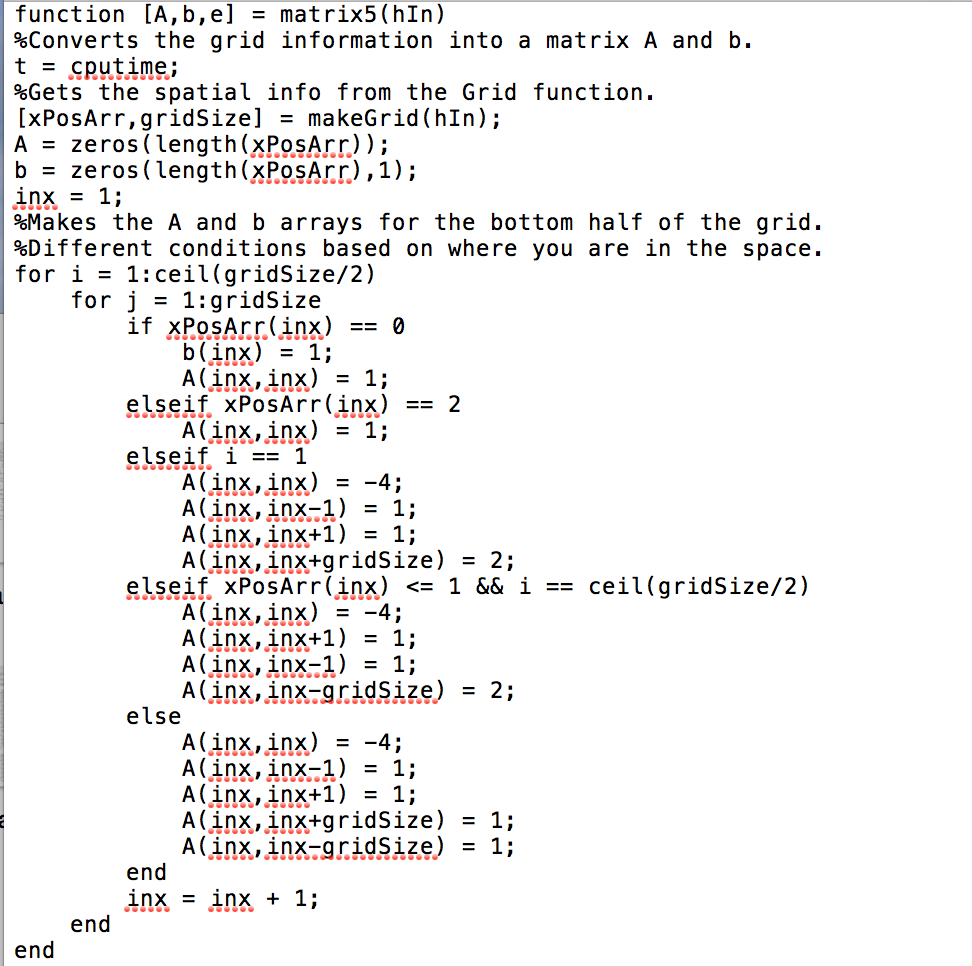
\includegraphics[scale = 0.7]{matrix5Code_1.png}} 

\centerline{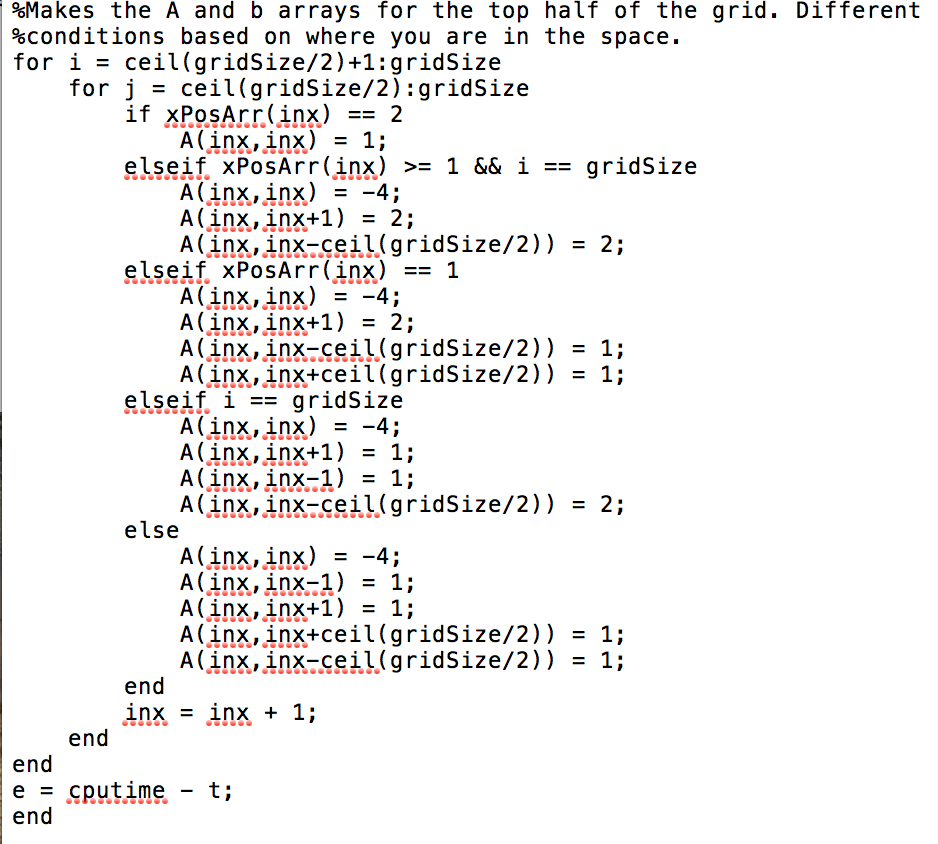
\includegraphics[scale = 0.7]{matrix5Code_2.png}} 

\section{Solving using Iterative Solvers}

Solve the resulting linear system using Jacobi, Gauss-Seidel, and Conjugate Gradient iterative solvers, and determine which solver worked best for this system. Solve the problem (from end- to-end) using several different values of h. Graph these results. Discuss the relationship between the number of elements and the time to solve the linear system. \\

Using prewritten Jacobi, Gauss-Seidel and Conjugate Gradient iterative solvers, I solved the linear system using the $A$ and $b$ matrices from the five-point stencil format for five different values of $h$. With the way I constructed my $A$ matrix, the conjugate gradient solver wouldn't converge so I chose to use the biconjugate gradient solver instead. The results of these iterative solvers are shown in the figures below. \\

Jacobi: \\

\centerline{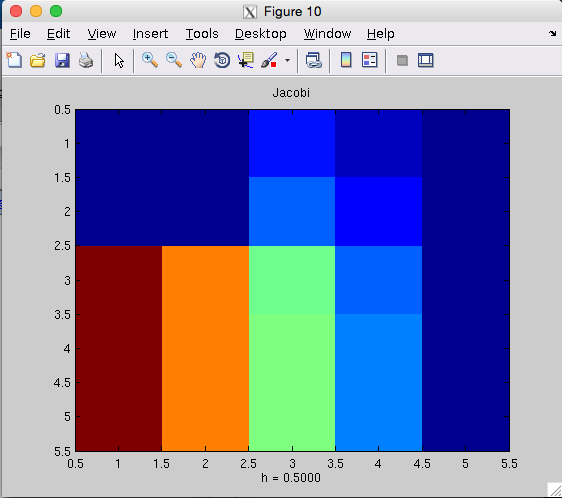
\includegraphics[scale = 0.55]{Jacobi_h1.png}}

\centerline{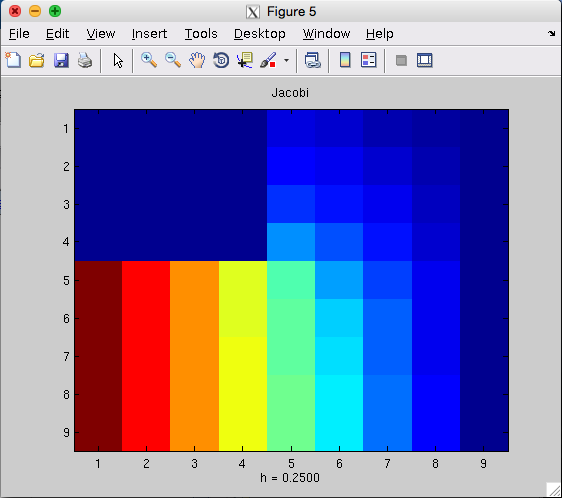
\includegraphics[scale = 0.55]{Jacobi_h2.png}}

\centerline{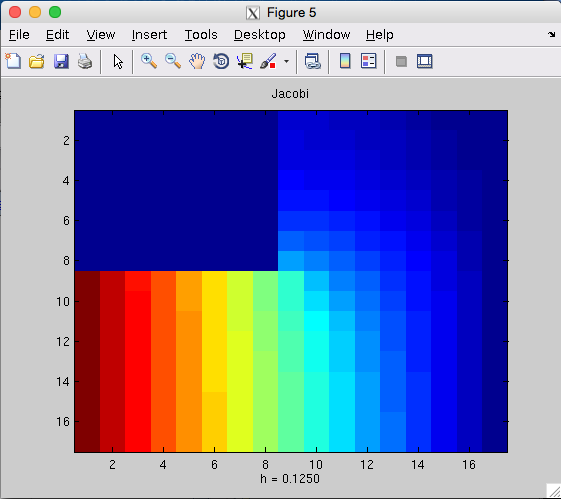
\includegraphics[scale = 0.55]{Jacobi_h3.png}}

\centerline{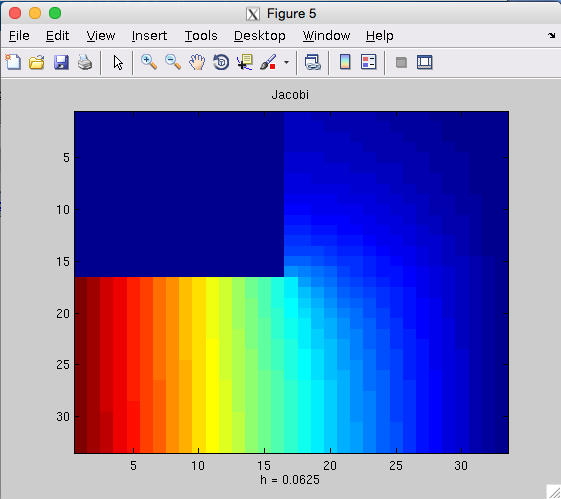
\includegraphics[scale = 0.55]{Jacobi_h4.png}}

\centerline{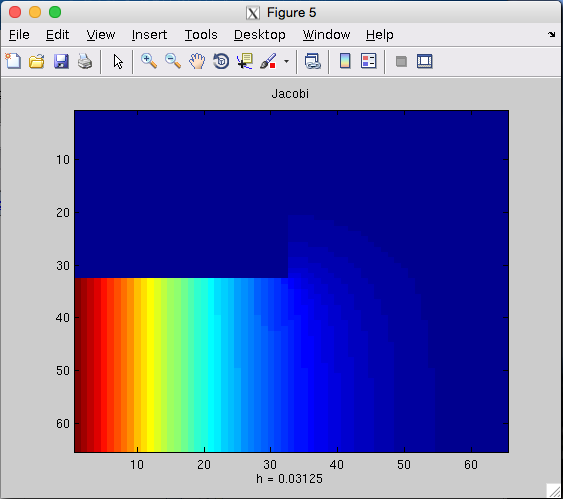
\includegraphics[scale = 0.55]{Jacobi_h5.png}}

Biconjugate Gradient: \\

\centerline{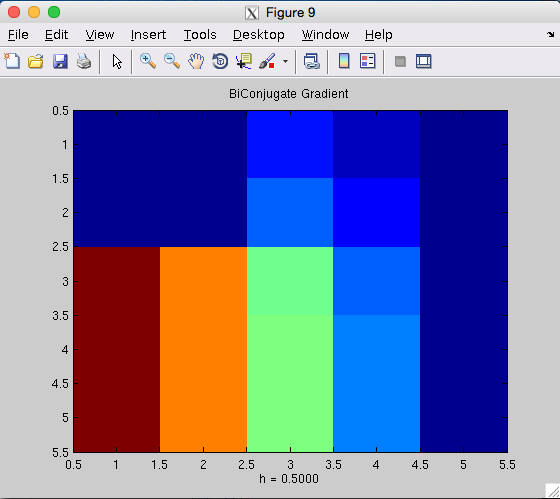
\includegraphics[scale = 0.55]{Biconjugate_h1.png}}

\centerline{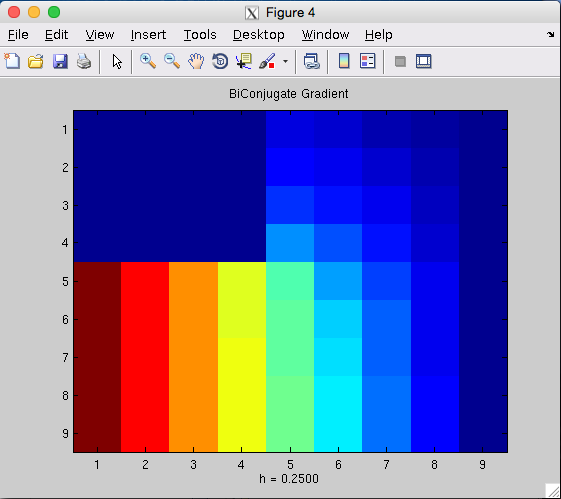
\includegraphics[scale = 0.55]{Biconjugate_h2.png}}

\centerline{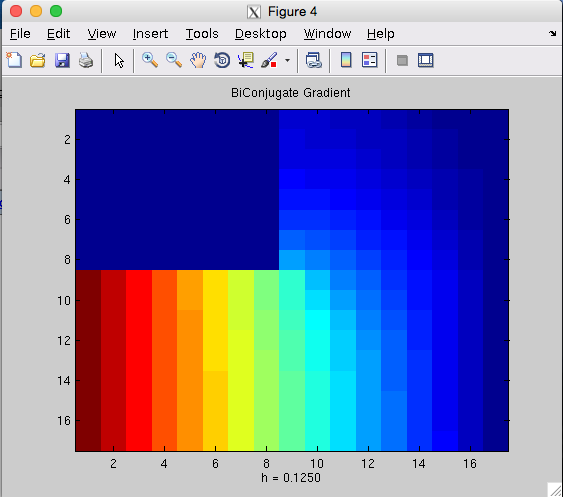
\includegraphics[scale = 0.55]{Biconjugate_h3.png}}

\centerline{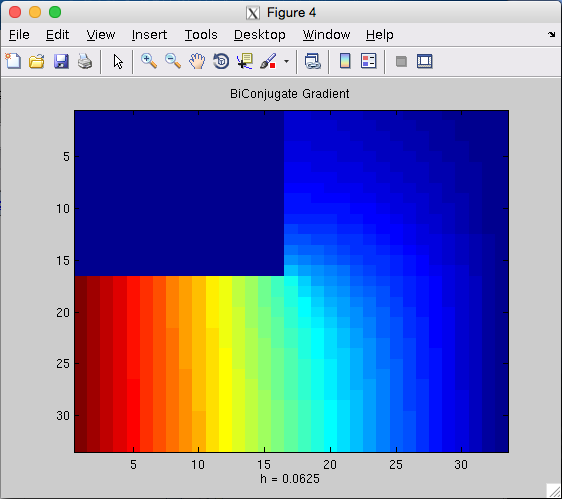
\includegraphics[scale = 0.55]{Biconjugate_h4.png}}

\centerline{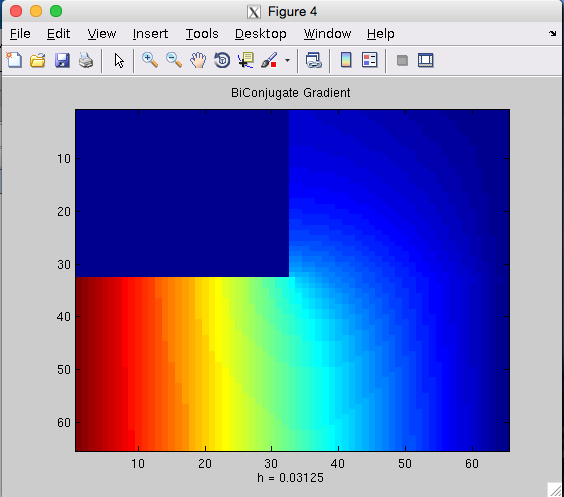
\includegraphics[scale = 0.55]{Biconjugate_h5.png}}

Gauss-Seidel: \\

\centerline{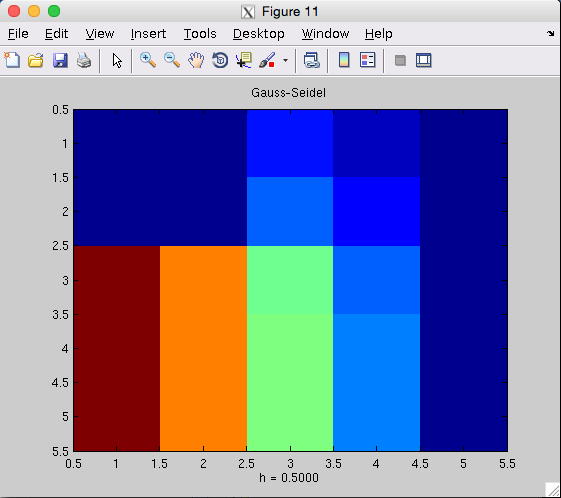
\includegraphics[scale = 0.55]{Gauss_h1.png}}

\centerline{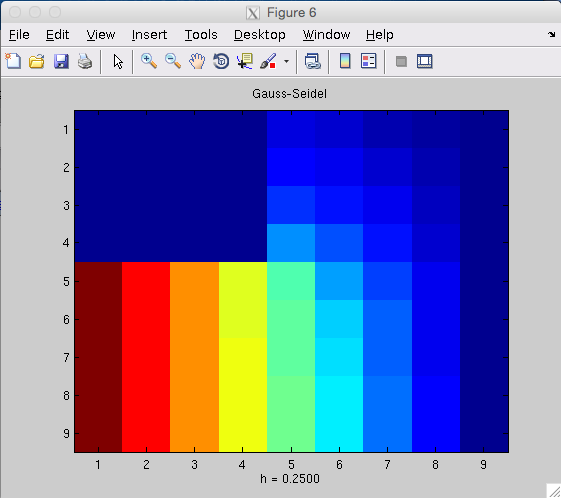
\includegraphics[scale = 0.55]{Gauss_h2.png}}

\centerline{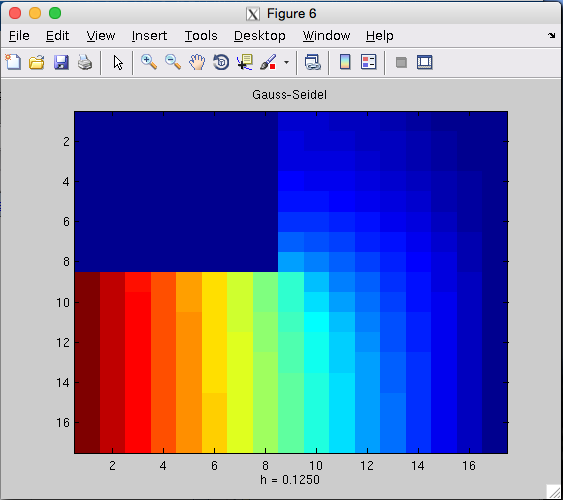
\includegraphics[scale = 0.55]{Gauss_h3.png}}

\centerline{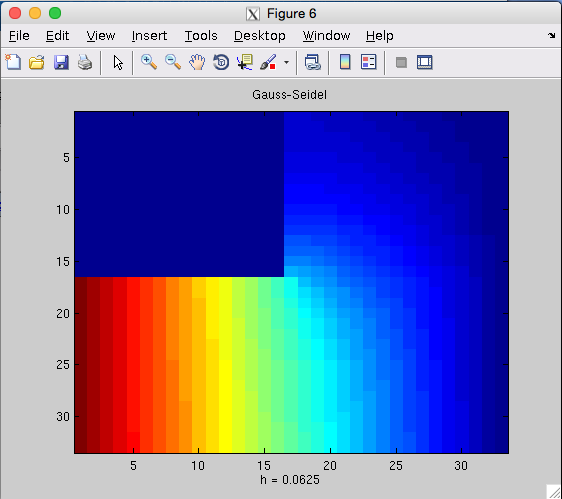
\includegraphics[scale = 0.55]{Gauss_h4.png}}

\centerline{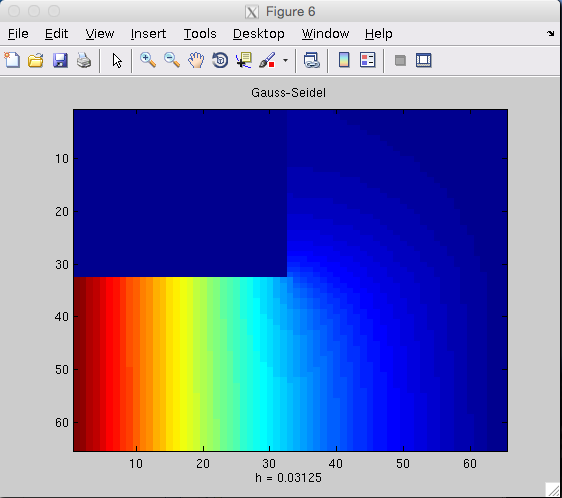
\includegraphics[scale = 0.55]{Gauss_h5.png}}

I also kept track of the CPU time for each of these methods for every value of $h$ shown in the table below. We can see that for every method as the number of elements increases so does the CPU time. We obtain our best results as the number of objects increases, but the computation time takes too long for any smaller values of $h$ than were tested in this experiment. Out of the three solvers that we tested, the Biconjugate Gradient solver was overall the fasted method and has the most visually pleasing solution. \\

\centerline{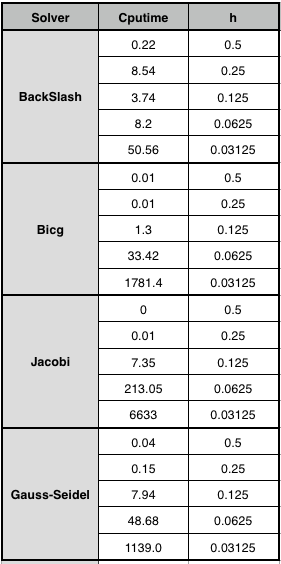
\includegraphics[scale = 0.75]{SolversComparisonTable.png}}

\section{Reworking Code to Solve a Linear System}

Rework your code so that it now uses the nine-point finite difference approximation for the Laplacian operator. Solve the previous problem (from end-to-end) using several different values of h. Again, graph the results. Compare the results from the nine-point and five-point difference formulas in terms of accuracy and computational costs. \\

In modifying my code into a nine-point stencil, different weights than the five-point stencil were applied to the current node and the eight surrounding nodes. The corner of the L also had to be slightly modified. The $A$ and $b$ matrices were built in the same fashion as the five-point stencil. After $A$ and $b$ were constructed, I used the backslash operator in MATLAB to quickly solve this linear system and visualize my results. The results were visualized for five different values of $h$ shown in the following figures. The code to create the stencil follows. \\

\centerline{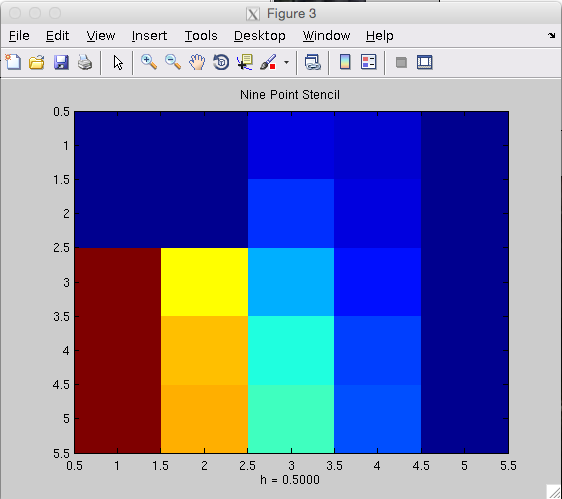
\includegraphics[scale = 0.55]{NinePoint_h1.png}}

\centerline{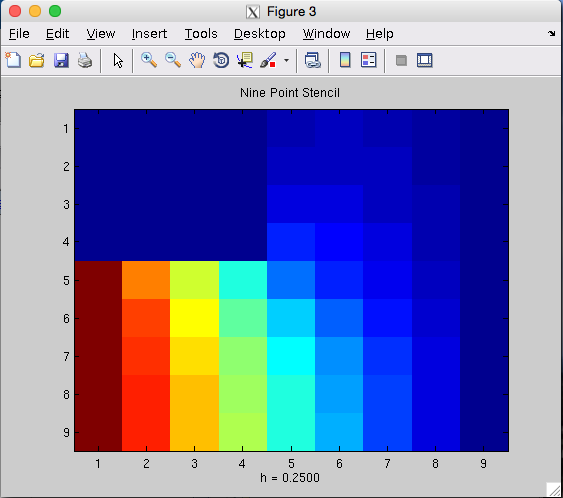
\includegraphics[scale = 0.55]{NinePoint_h2.png}}

\centerline{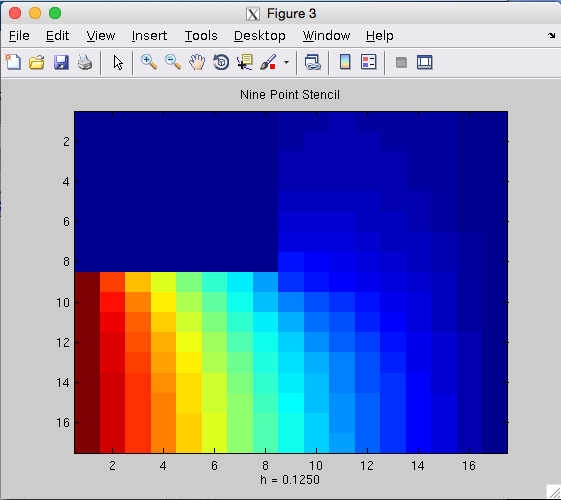
\includegraphics[scale = 0.55]{NinePoint_h3.png}}

\centerline{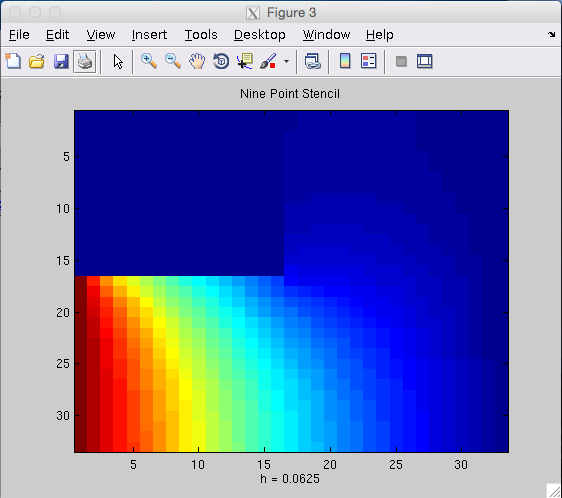
\includegraphics[scale = 0.55]{NinePoint_h4.png}}

\centerline{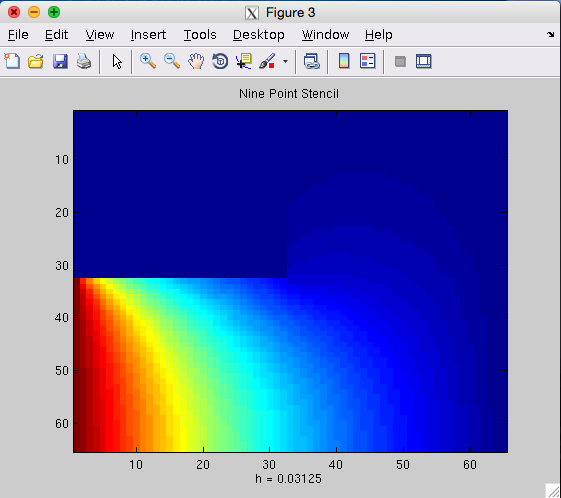
\includegraphics[scale = 0.55]{NinePoint_h5.png}}

\centerline{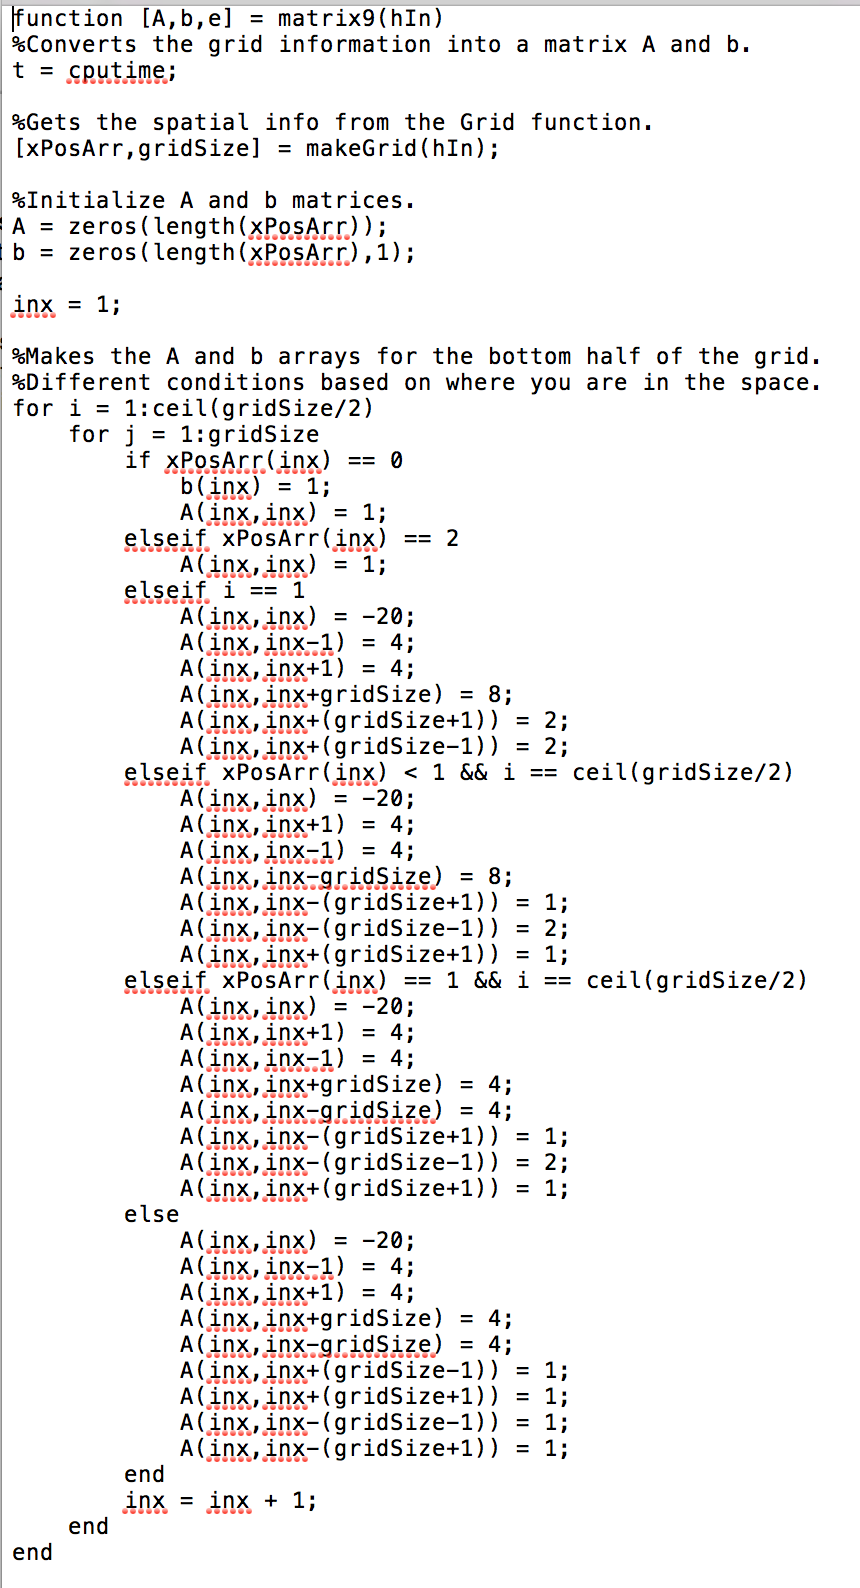
\includegraphics[scale = 0.7]{matrix9Code_1.png}} 

\centerline{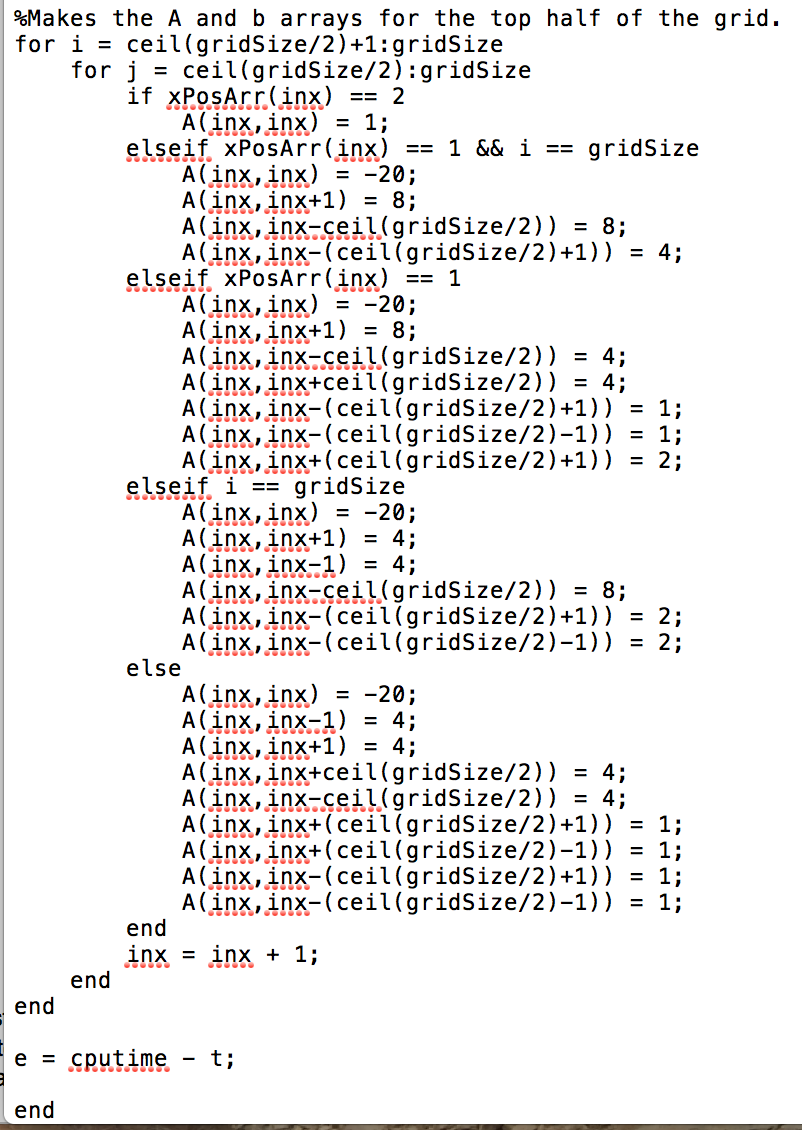
\includegraphics[scale = 0.7]{matrix9Code_2.png}} 

I also kept track of the CPU time for both the five-point and the nine-point stencil for every value of $h$ shown in the table below. These results were surprising in the beginning because the nine-point stencil is faster than the five-point, but as the number of elements increases the CPU time between the two methods gets closer together. I would assume that there is a certain number of elements were the five-point stencil is consistently faster than the nine-point stencil. We can see from the images that the nine-point stencil is a better solution. \\

\centerline{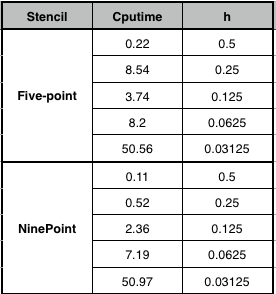
\includegraphics[scale = 0.75]{5vs9Table.png}}

*All of the code for this assignment is included in the submission.

\end{document}  